\documentclass[UTF8]{article}
\usepackage{arxiv}
\usepackage{ctex}
\usepackage[utf8]{inputenc} % allow utf-8 input
\usepackage[T1]{fontenc} % use 8-bit T1 fonts
\usepackage{url} % simple URL typesetting
\usepackage{booktabs} % professional-quality tables
\usepackage{amsfonts,amsmath,amssymb} % blackboard math symbols
\usepackage{nicefrac} % compact symbols for 1/2, etc.
\usepackage{microtype} % microtypography
\usepackage{lipsum} % Can be removed after putting your text content
\usepackage{graphicx}
\usepackage{natbib}
\usepackage{doi}
\usepackage{fontspec}
\usepackage{caption}
\usepackage{hyperref} % hyperlinks for references
\hypersetup{hidelinks,
colorlinks=true,
linkcolor=red,
citecolor=green
}


\title{大数据中的案例实务课程报告}
\author{
    {\hspace{1mm}张三} \\
    大数据学院\\
    \texttt{25210980000@m.fudan.edu.cn} \\
}


\renewcommand{\headeright}{Report}
\renewcommand{\shorttitle}{MAS60001 大数据中的案例实务}
\setlength{\parindent}{2em}
\setmainfont{Times New Roman}

\begin{document}
\maketitle


% ============= ABSTRACT ============= %
\begin{abstract}
这是一段摘要。简明地概括这份报告的背景、方法、主要结果和结论。字数建议在 250-350 字之间。
\end{abstract}
\keywords{关键词1 \and 关键词2 \and 关键词3}

% ============= INTRODUCTION ============= %
\section{引言}\label{sec:introduction}
这篇模板仅作为一个粗糙的框架以供参考，你可以自由地组织各个章节、子章节的标题和内容。

引言部分的目的是为读者提供一个研究背景和目标的概述，让读者熟悉一些必要的背景知识，激发读者的兴趣，并引导他们阅读论文的后续部分。由于本文是一份课程报告，因此背景信息不必太过详细，例如：

\begin{itemize}
    \item 介绍所研究问题的背景；
    \item 简单概述研究所采用的基本方法；
    \item 明确研究的目的和意义。
\end{itemize}


% ============= METHODOLOGY ============= %
\section{方法}\label{sec:methodology}
介绍你在这项研究中所采用的方法。在阐述方法细节之前，建议明确方法的设计思想——“为什么要用这个方法？”、“方法中采用这个模块的目的是什么？”。若方法包含了多个步骤或者多个模块，可以分出多个子章节介绍。

在描述过程中，有时你可能需要展示一些图（例如图~\ref{fig:em}），用到一些数学符号~\cite{downes2002short}（如$\alpha$, $\beta$等），行内公式（如$\bar{x} = \frac{1}{n}\sum_{i=1}^{n}x_i$），或者如式~\eqref{eq:gaussian}所示的行间公式~\cite{do2008multivariate}：
\begin{equation}
    g(\boldsymbol{x}) = 
    \dfrac{1}
    {(2\pi)^{n/2}
    \left|\boldsymbol{\Sigma}\right|^{1/2}}
    \exp
    \left[
    -\dfrac{1}{2}
    (\boldsymbol{x-\mu})^\top
    \boldsymbol{\Sigma}^{-1}
    (\boldsymbol{x-\mu})
    \right],
    \label{eq:gaussian}
\end{equation}

以及如式~\eqref{eq:em-alg}所示的多个子公式~\cite{moon1996em}。更多的\LaTeX 符号及其用法请参考文献~\cite{downes2002short}：
\begin{subequations}
\begin{align}
    \theta^{(t+1)} &=
    \underset{\theta}{\arg\max}
    \int_Z
    \log P(X,Z|\theta) 
    P\left( Z|X,\theta^{(t)} \right)
    \mathrm{d}Z,
    \label{eq:em}\\
    P\left( Z|X,\theta^{(t)} \right) &\rightarrow
    \mathbb{E}_{Z|X, \theta^{(t)}}
    [\log P(X,Z|\theta)],
    \label{eq:e-step}\\
    \theta^{(t+1)} &=
    \underset{\theta}{\arg\max}
    \left\{
    \mathbb{E}_{Z|X, \theta^{(t)}}
    \left[\log P(X,Z|\theta)\right]
    \right\}.
    \label{eq:m-step}
\end{align}
\label{eq:em-alg}
\end{subequations}


\begin{figure}[!htb]
    \centering
    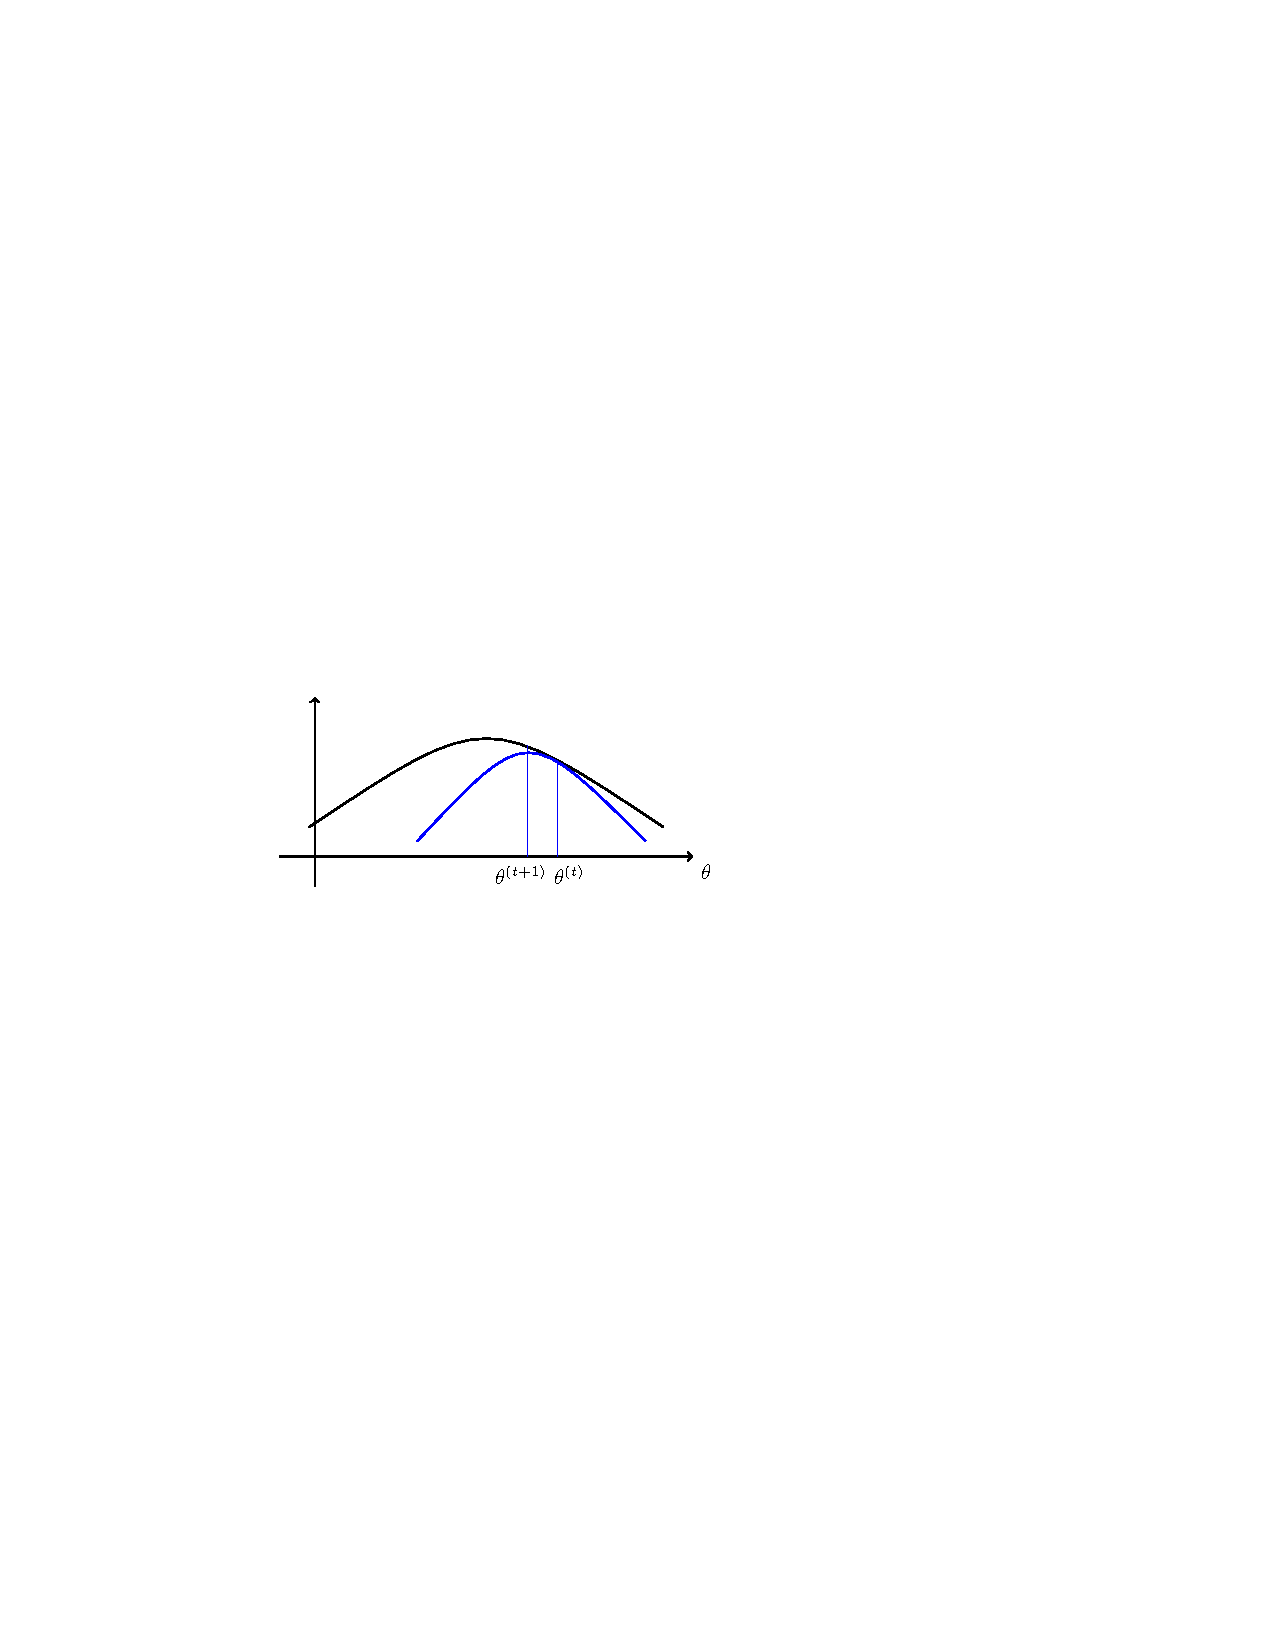
\includegraphics[width=\linewidth]{figs/em.pdf}
    \captionsetup{font={small,bf}}  % 小号加粗
    \caption{EM算法示意图。}
    \label{fig:em}
\end{figure}

\subsection{模块1}
介绍模块1。
\subsubsection{子模块1}
介绍子模块1。

\subsection{模块2}
介绍模块2。




% ============= EXPERIMENTS ============= %
\section{实验}\label{sec:experiments}
\subsection{数据集}
对所采用的数据集进行介绍。

\subsection{实验设定}
对其他实验设定进行介绍，如实验内容、硬件、软件、相关超参数设定等。

% ============= RESULTS ============= %
\section{结果与分析}\label{sec:results}
通过图和表等方式展示各项实验的结果，如表~\ref{tab:sample}和图~\ref{fig:sample}所示，并对其进行分析和讨论。
\begin{table}[!htb]
    \centering
    \captionsetup{font={small,bf}} % 小号加粗, 位于表格上方
    \caption{样例表格。}
    \begin{tabular}{cccccc}  % 'c'enter for 6 columns
    \toprule
    variants & SVCT-PSNR & SVCT-SSIM & LACT-PSNR & LACT-SSIM \\
    \midrule
    V1 & \textbf{40.00} & \textbf{98.88} & 39.99 & 94.44 \\
    V2 & 38.88 & 95.55 & \textbf{41.11} & \textbf{96.66} \\
    \bottomrule
    \end{tabular}
    \label{tab:sample}
\end{table}


\begin{figure}[!htb]
    \centering
    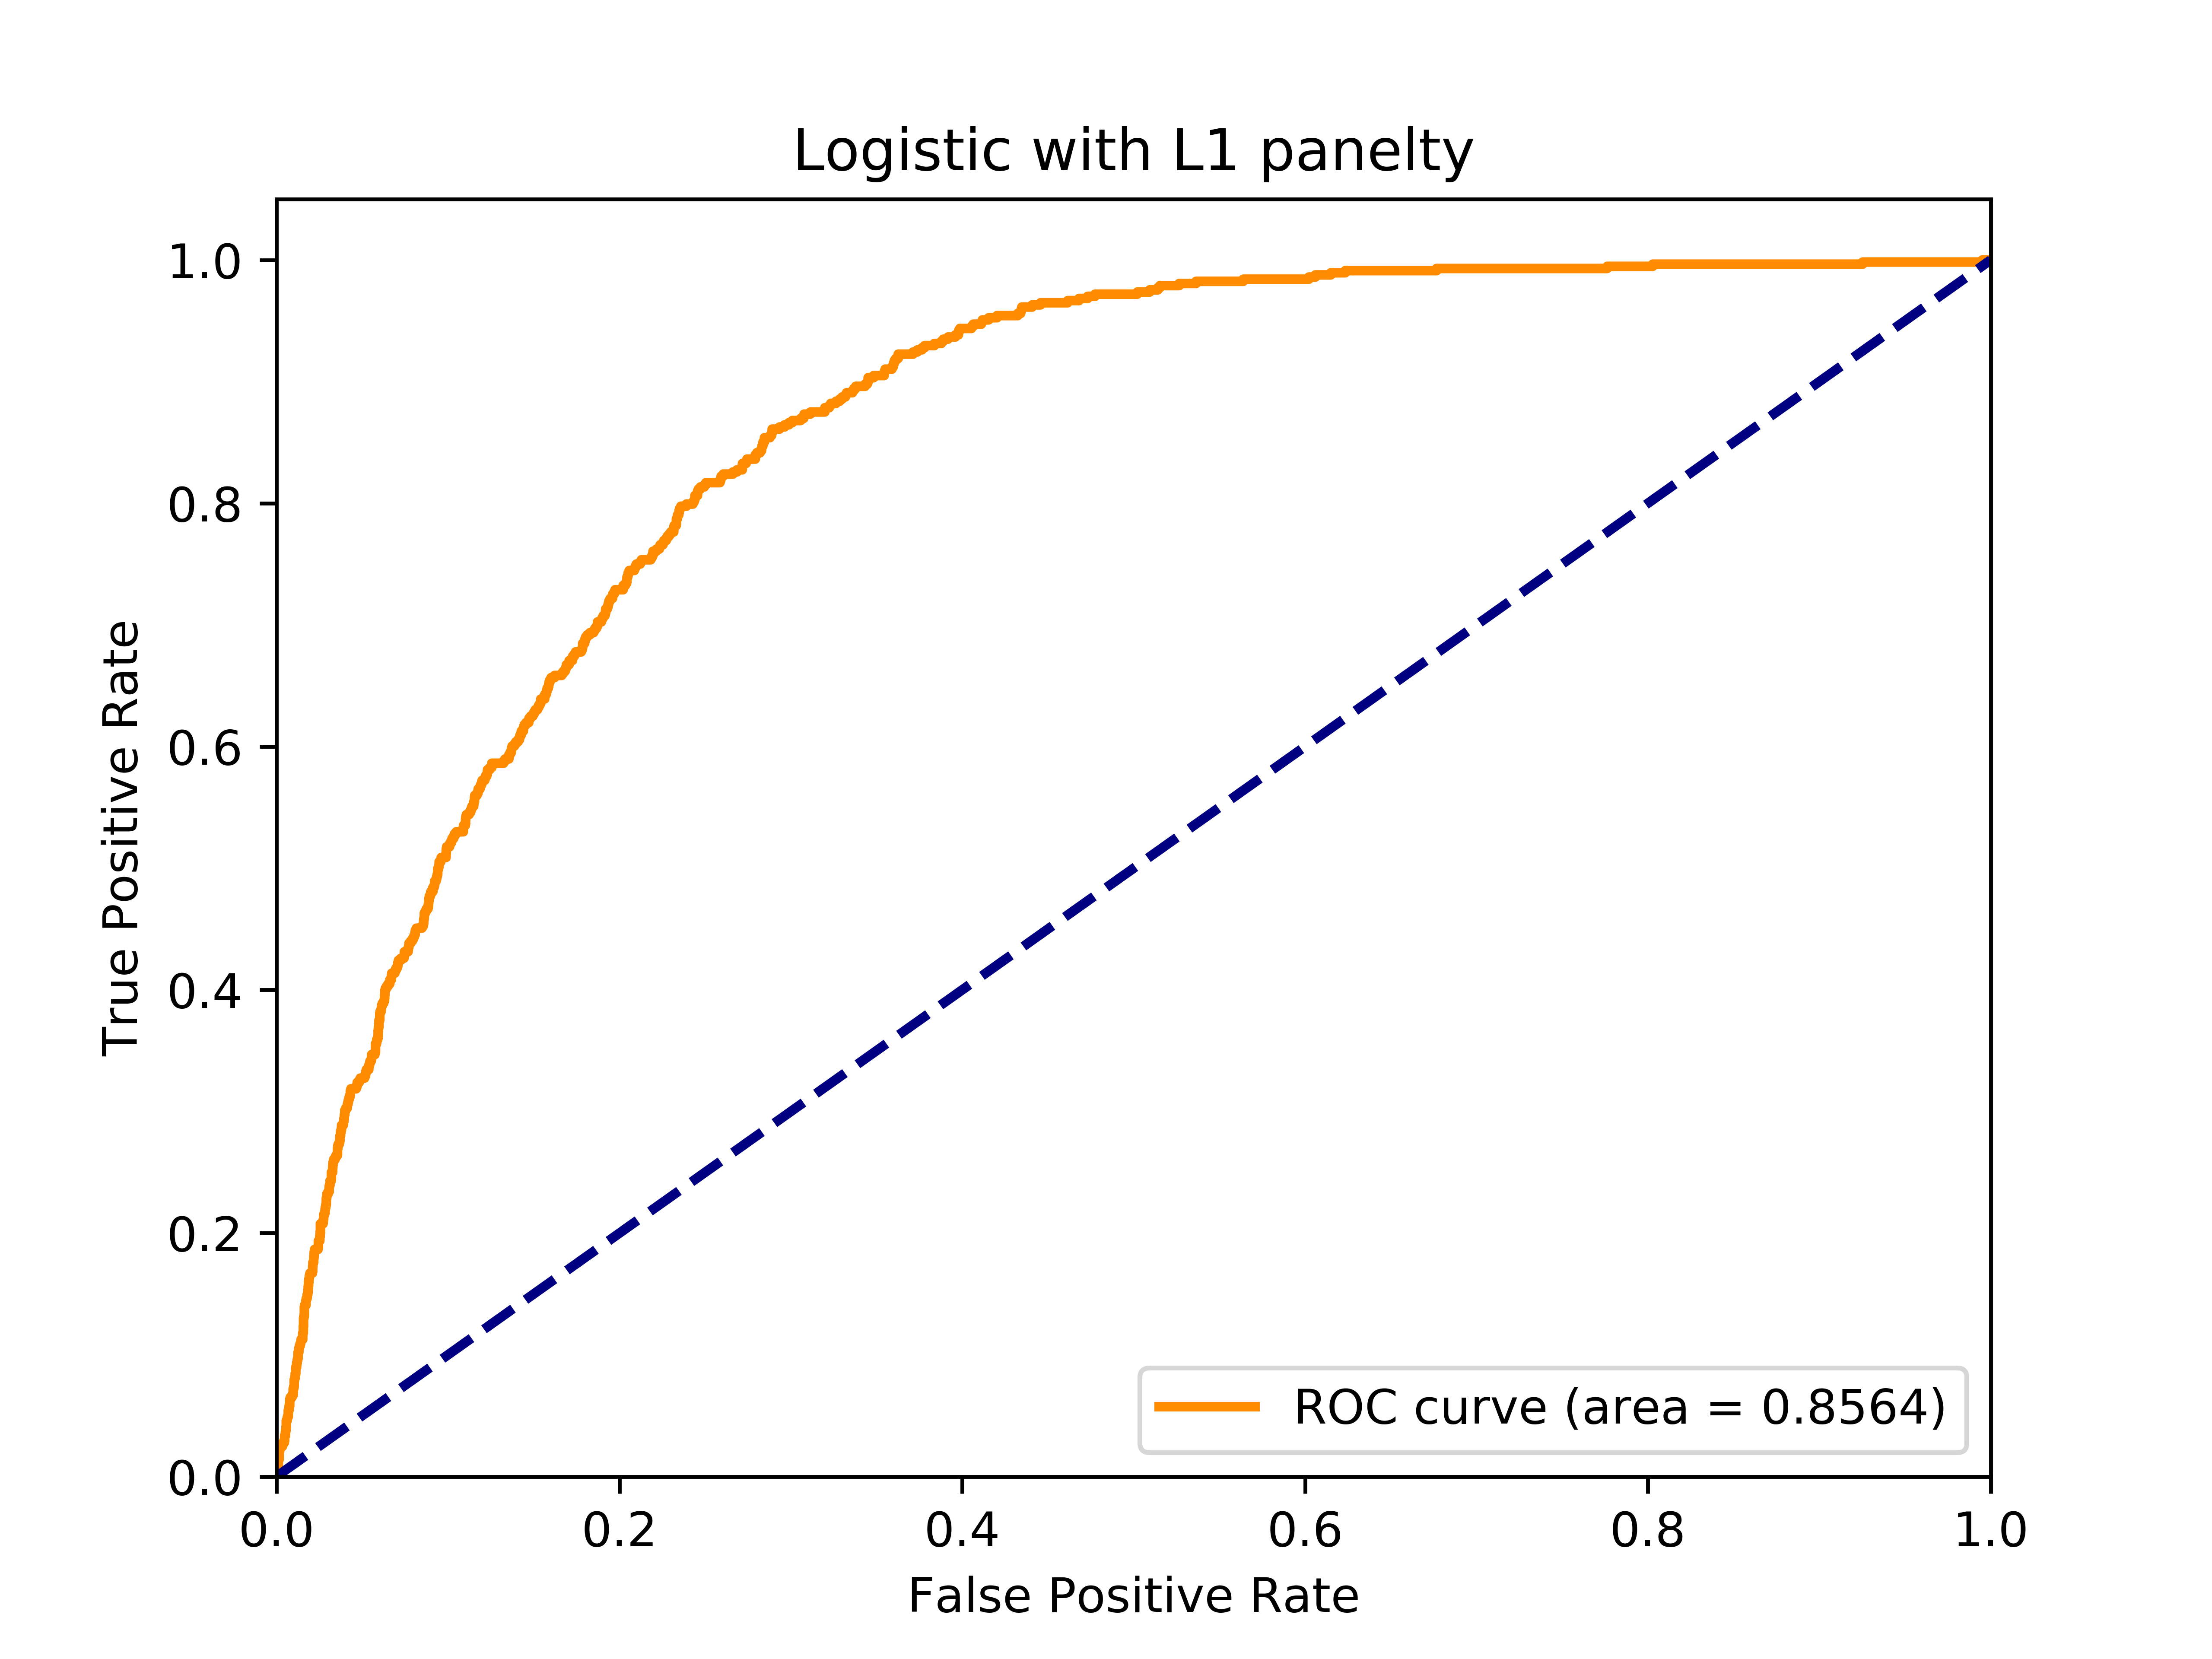
\includegraphics[width=0.5\linewidth]{figs/sample.png}
    \captionsetup{font={small,bf}}  % 小号加粗
    \caption{样例图片。}
    \label{fig:sample}
\end{figure}


% ============= CONCLUSION ============= %
\section{结论}\label{sec:conclusion}
总结整份报告，归纳出结论。



% ============= REFERENCES ============= %
\bibliographystyle{unsrt}
% You can directly copy the Bibtex of the cited literature to the references.bib file, and run the following line to generate the bibliography automatically:
\bibliography{references}  

% But if you want to write the bibliography on you own, uncomment the above line and comment out the ``thebibliography'' section below to use the external .bib file (using bibtex) .

%%% Uncomment this section and comment out the \bibliography{references} line above to use inline references.
% \begin{thebibliography}{1}

% 	\bibitem{kour2014real}
% 	George Kour and Raid Saabne.
% 	\newblock Real-time segmentation of on-line handwritten arabic script.
% 	\newblock In {\em Frontiers in Handwriting Recognition (ICFHR), 2014 14th
% 			International Conference on}, pages 417--422. IEEE, 2014.

% 	\bibitem{kour2014fast}
% 	George Kour and Raid Saabne.
% 	\newblock Fast classification of handwritten on-line arabic characters.
% 	\newblock In {\em Soft Computing and Pattern Recognition (SoCPaR), 2014 6th
% 			International Conference of}, pages 312--318. IEEE, 2014.

% 	\bibitem{hadash2018estimate}
% 	Guy Hadash, Einat Kermany, Boaz Carmeli, Ofer Lavi, George Kour, and Alon
% 	Jacovi.
% 	\newblock Estimate and replace: A novel approach to integrating deep neural
% 	networks with existing applications.
% 	\newblock {\em arXiv preprint arXiv:1804.09028}, 2018.

% \end{thebibliography}


% If you need an appendix, uncomment the following three lines:
% \newpage
% \appendix
% \section*{附录}


\end{document}
